
\begin{figure}[!h]
    \centering
    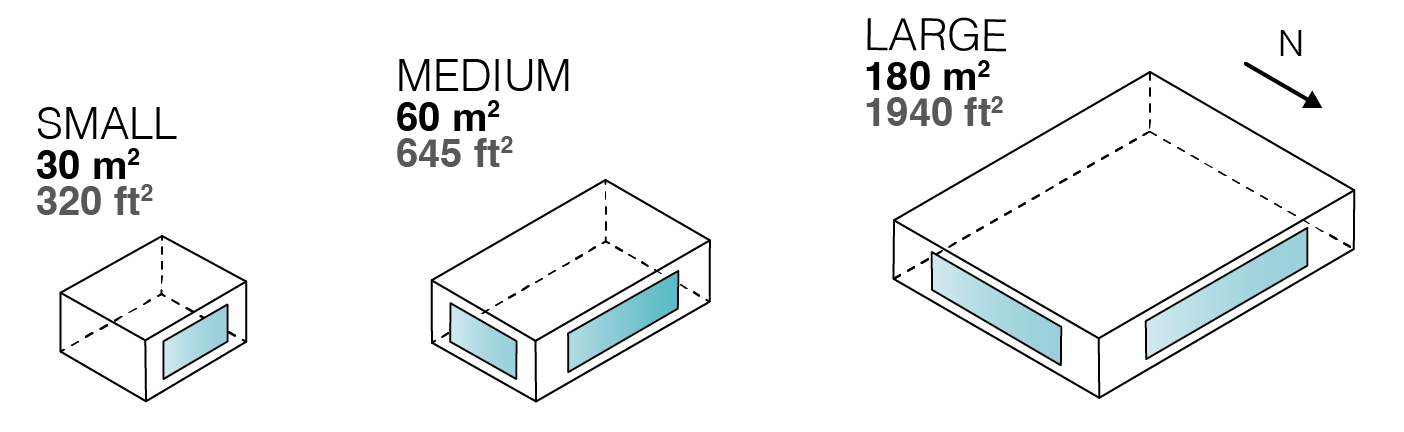
\includegraphics[width=0.8\textwidth]{manuscript/src/figures/scenario-size.png}
    \vspace{0.5cm}
    % \caption{Geometry of case study model.}

        \renewcommand{\arraystretch}{1.25}
    

        \begin{tabular}{ p{3.5cm} p{2cm} p{2cm} p{2cm} }
        
            \hline
            
            {\textbf{Setting(s)}} & \multicolumn{3}{l}{\textbf{Definition}} \\
        
            \hline
        
            {Climates}  & \multicolumn{3}{l}{Sydney, Australia (Cfa), TMY \& 2070 (RCP 4.5)} \\
        
            % \cline{2-3}
            
            {Constructions} & \multicolumn{3}{l}{\textit{ASHRAE 90.1 2019, IECC 2021}, Steel-framed*} \\
        
            % \cline{2-3}  
            
            {Program} & \multicolumn{3}{l}{\textit{Small Office*}} \\
            
            % \cline{2-3}
        
            {HVAC system} & \multicolumn{3}{l}{IdealAir system, Air conditioned} \\
        
            % \cline{2-3}

            {Passive Design Level} & {a) \textbf{Standard}} & {b) \textbf{Medium}} & {c) \textbf{Advanced}} \\

            \cline{2-4}
        
            {Natural Ventilation?} & {No} & {Yes} & {Yes} \\
        

            {Envelope} & {$U_{win} = 2.0$\newline $U_{wall} = 0.35$\newline $WWR = 0.4$ \newline No shading} & {$U_{win} = 1.3$\newline $U_{wall} = 0.2$\newline $WWR = 0.3$ \newline No shading} & {$U_{win} = 1.3$\newline $U_{wall} = 0.2$\newline $WWR = 0.3$ \newline Ext. shading} \\

             % \cline{2-3}
        
            {AC* setpoint range\newline \textit{Heating - Cooling}} & {22-24\degree C} & {22-24\degree C} & {22-24\degree C} \\
            
            \hline
        
        \end{tabular}
        \vspace{0.5cm}
        \caption{Overview of main settings for simulated case study scenarios: Construction properties, loads and schedules were based on Department of Energy (DOE) reference building information. (AC* - Air Conditioning (if used), WWR - Window-to-Wall-Ratio, U - U value in W/m²K)}
        \label{tab:sim-settings}
        

\end{figure}